\documentclass[letterpaper]{article}

\usepackage{tikz}
\usepackage{subcaption}
\usepackage{float}


\begin{document}
\section{Examples}

\subsection{Example 1: Mediator model ($ X \rightarrow M \rightarrow Y $):} All effects = $ 0.3 $. Left marginal correlation, right conditional

\begin{figure}[H]
	\centering
	\begin{subfigure}{0.5 \textwidth}
		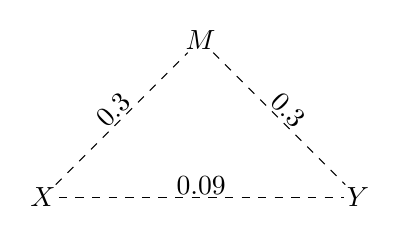
\begin{tikzpicture}[scale=2]
				\tikzstyle{every node}=[inner sep=1pt, align=center]
				\node (X) at (0, 0) {$ X $};
				\node (M) at (1, 1) {$ M $};
				\node (Y) at (2, 0) {$ Y $};
				\draw [dashed] (X) -- (M) node[midway, above, sloped] {$0.3$};
				\draw [dashed] (M) -- (Y) node[midway, above, sloped] {$0.3$};
				\draw [dashed] (X) -- (Y) node[midway, above, sloped] {$0.09$};
		\end{tikzpicture}
	\end{subfigure}%
	\begin{subfigure}{0.5 \textwidth}
		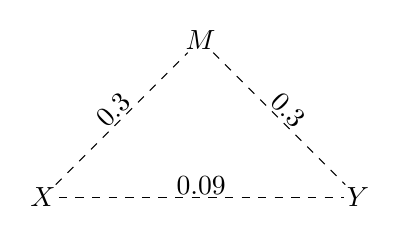
\begin{tikzpicture}[scale=2]
				\tikzstyle{every node}=[inner sep=1pt, align=center]
				\node (X) at (0, 0) {$ X $};
				\node (M) at (1, 1) {$ M $};
				\node (Y) at (2, 0) {$ Y $};
				\draw [dashed] (X) -- (M) node[midway, above, sloped] {$0.3$};
				\draw [dashed] (M) -- (Y) node[midway, above, sloped] {$0.3$};
				\draw [dashed] (X) -- (Y) node[midway, above, sloped] {$0.09$};
		\end{tikzpicture}
	\end{subfigure}
\end{figure}

Add edge $ M \rightarrow Y $:

\begin{figure}[H]
	\centering
	\begin{subfigure}{0.5 \textwidth}
		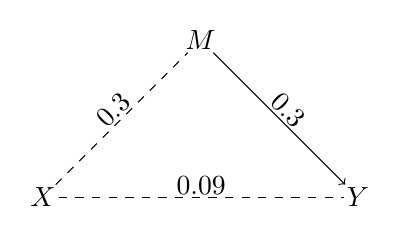
\begin{tikzpicture}[scale=2]
				\tikzstyle{every node}=[inner sep=1pt, align=center]
				\node (X) at (0, 0) {$ X $};
				\node (M) at (1, 1) {$ M $};
				\node (Y) at (2, 0) {$ Y $};
				\draw [dashed] (X) -- (M) node[midway, above, sloped] {$0.3$};
				\draw [->] (M) -- (Y) node[midway, above, sloped] {$0.3$};
				\draw [dashed] (X) -- (Y) node[midway, above, sloped] {$0.09$};
		\end{tikzpicture}
	\end{subfigure}%
	\begin{subfigure}{0.5 \textwidth}
		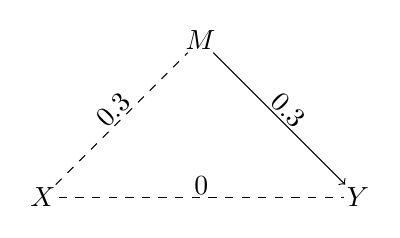
\begin{tikzpicture}[scale=2]
				\tikzstyle{every node}=[inner sep=1pt, align=center]
				\node (X) at (0, 0) {$ X $};
				\node (M) at (1, 1) {$ M $};
				\node (Y) at (2, 0) {$ Y $};
				\draw [dashed] (X) -- (M) node[midway, above, sloped] {$0.3$};
				\draw [->] (M) -- (Y) node[midway, above, sloped] {$0.3$};
				\draw [dashed] (X) -- (Y) node[midway, above, sloped] {$0$};
		\end{tikzpicture}
	\end{subfigure}
\end{figure}

Add edge $ X \rightarrow M $:

\begin{figure}[H]
	\centering
	\begin{subfigure}{0.5 \textwidth}
		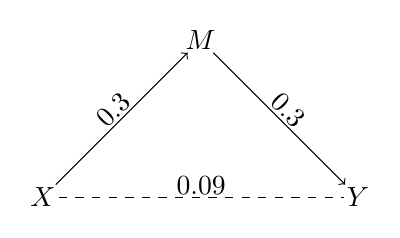
\begin{tikzpicture}[scale=2]
				\tikzstyle{every node}=[inner sep=1pt, align=center]
				\node (X) at (0, 0) {$ X $};
				\node (M) at (1, 1) {$ M $};
				\node (Y) at (2, 0) {$ Y $};
				\draw [->] (X) -- (M) node[midway, above, sloped] {$0.3$};
				\draw [->] (M) -- (Y) node[midway, above, sloped] {$0.3$};
				\draw [dashed] (X) -- (Y) node[midway, above, sloped] {$0.09$};
		\end{tikzpicture}
	\end{subfigure}%
	\begin{subfigure}{0.5 \textwidth}
		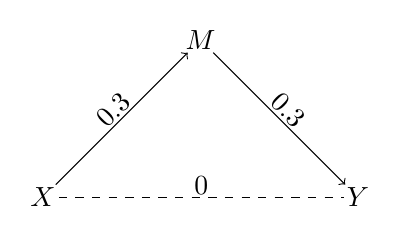
\begin{tikzpicture}[scale=2]
				\tikzstyle{every node}=[inner sep=1pt, align=center]
				\node (X) at (0, 0) {$ X $};
				\node (M) at (1, 1) {$ M $};
				\node (Y) at (2, 0) {$ Y $};
				\draw [->] (X) -- (M) node[midway, above, sloped] {$0.3$};
				\draw [->] (M) -- (Y) node[midway, above, sloped] {$0.3$};
				\draw [dashed] (X) -- (Y) node[midway, above, sloped] {$0$};
		\end{tikzpicture}
	\end{subfigure}
\end{figure}

Add edge $ X \rightarrow Y $ in the marginal case:

\begin{figure}[H]
	\centering
	\begin{subfigure}{0.5 \textwidth}
		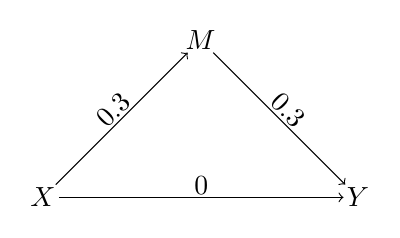
\begin{tikzpicture}[scale=2]
				\tikzstyle{every node}=[inner sep=1pt, align=center]
				\node (X) at (0, 0) {$ X $};
				\node (M) at (1, 1) {$ M $};
				\node (Y) at (2, 0) {$ Y $};
				\draw [->] (X) -- (M) node[midway, above, sloped] {$0.3$};
				\draw [->] (M) -- (Y) node[midway, above, sloped] {$0.3$};
				\draw [->] (X) -- (Y) node[midway, above, sloped] {$0$};
		\end{tikzpicture}
	\end{subfigure}
	\begin{subfigure}{0.5 \textwidth}
	\end{subfigure}
\end{figure}

\subsection{Example 2: Mediator with edge $ X \rightarrow Y $}

Add edge $ M \rightarrow Y $:

\begin{figure}[H]
	\centering
	\begin{subfigure}{0.5 \textwidth}
		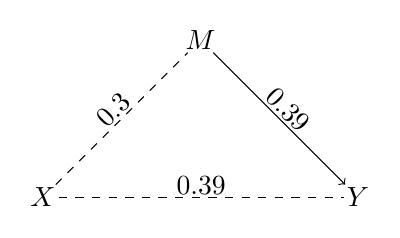
\begin{tikzpicture}[scale=2]
				\tikzstyle{every node}=[inner sep=1pt, align=center]
				\node (X) at (0, 0) {$ X $};
				\node (M) at (1, 1) {$ M $};
				\node (Y) at (2, 0) {$ Y $};
				\draw [dashed] (X) -- (M) node[midway, above, sloped] {$0.3$};
				\draw [->] (M) -- (Y) node[midway, above, sloped] {$0.39$};
				\draw [dashed] (X) -- (Y) node[midway, above, sloped] {$0.39$};
		\end{tikzpicture}
	\end{subfigure}%
	\begin{subfigure}{0.5 \textwidth}
		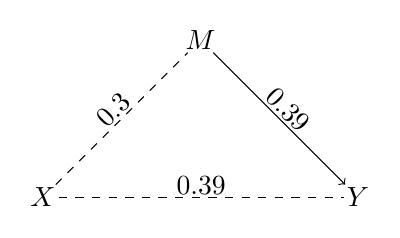
\begin{tikzpicture}[scale=2]
				\tikzstyle{every node}=[inner sep=1pt, align=center]
				\node (X) at (0, 0) {$ X $};
				\node (M) at (1, 1) {$ M $};
				\node (Y) at (2, 0) {$ Y $};
				\draw [dashed] (X) -- (M) node[midway, above, sloped] {$0.3$};
				\draw [->] (M) -- (Y) node[midway, above, sloped] {$0.39$};
				\draw [dashed] (X) -- (Y) node[midway, above, sloped] {$0.39$};
		\end{tikzpicture}
	\end{subfigure}
\end{figure}

Add edge $ X \rightarrow Y $:

\begin{figure}[H]
	\centering
	\begin{subfigure}{0.5 \textwidth}
		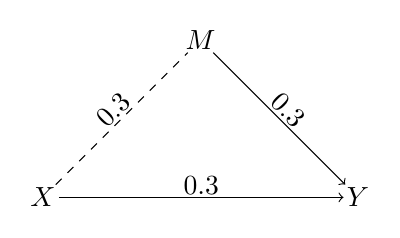
\begin{tikzpicture}[scale=2]
				\tikzstyle{every node}=[inner sep=1pt, align=center]
				\node (X) at (0, 0) {$ X $};
				\node (M) at (1, 1) {$ M $};
				\node (Y) at (2, 0) {$ Y $};
				\draw [dashed] (X) -- (M) node[midway, above, sloped] {$0.3$};
				\draw [->] (M) -- (Y) node[midway, above, sloped] {$0.3$};
				\draw [->] (X) -- (Y) node[midway, above, sloped] {$0.3$};
		\end{tikzpicture}
	\end{subfigure}%
	\begin{subfigure}{0.5 \textwidth}
		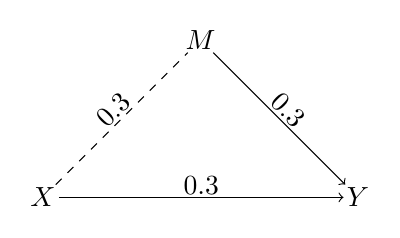
\begin{tikzpicture}[scale=2]
				\tikzstyle{every node}=[inner sep=1pt, align=center]
				\node (X) at (0, 0) {$ X $};
				\node (M) at (1, 1) {$ M $};
				\node (Y) at (2, 0) {$ Y $};
				\draw [dashed] (X) -- (M) node[midway, above, sloped] {$0.3$};
				\draw [->] (M) -- (Y) node[midway, above, sloped] {$0.3$};
				\draw [->] (X) -- (Y) node[midway, above, sloped] {$0.3$};
		\end{tikzpicture}
	\end{subfigure}
\end{figure}

Add edge $ X \rightarrow M $:

\begin{figure}[H]
	\centering
	\begin{subfigure}{0.5 \textwidth}
		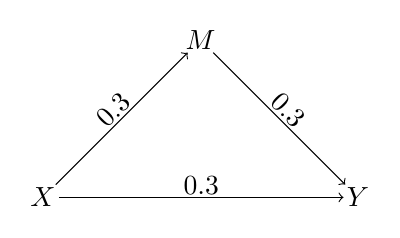
\begin{tikzpicture}[scale=2]
				\tikzstyle{every node}=[inner sep=1pt, align=center]
				\node (X) at (0, 0) {$ X $};
				\node (M) at (1, 1) {$ M $};
				\node (Y) at (2, 0) {$ Y $};
				\draw [->] (X) -- (M) node[midway, above, sloped] {$0.3$};
				\draw [->] (M) -- (Y) node[midway, above, sloped] {$0.3$};
				\draw [->] (X) -- (Y) node[midway, above, sloped] {$0.3$};
		\end{tikzpicture}
	\end{subfigure}%
	\begin{subfigure}{0.5 \textwidth}
		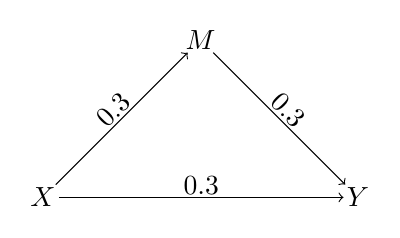
\begin{tikzpicture}[scale=2]
				\tikzstyle{every node}=[inner sep=1pt, align=center]
				\node (X) at (0, 0) {$ X $};
				\node (M) at (1, 1) {$ M $};
				\node (Y) at (2, 0) {$ Y $};
				\draw [->] (X) -- (M) node[midway, above, sloped] {$0.3$};
				\draw [->] (M) -- (Y) node[midway, above, sloped] {$0.3$};
				\draw [->] (X) -- (Y) node[midway, above, sloped] {$0.3$};
		\end{tikzpicture}
	\end{subfigure}
\end{figure}

Remarks:
\begin{enumerate}
	\item After drawing an edge, the parameter values can change. Happens in both cases.
	\item In the marginal case, all paths between variables with effect get added and later need to be pruned. Pruning is required in the conditional case as well.
\end{enumerate}

\end{document}
